\documentclass[11pt,fleqn]{article}

\usepackage{blindtext}
\usepackage{hyperref}
\usepackage{graphicx}

\graphicspath{ {./} }

\hypersetup{
    colorlinks=true,
    linkcolor=blue,
    filecolor=magenta,      
    urlcolor=cyan,
    pdftitle={Overleaf Example},
    pdfpagemode=FullScreen,
    }
\urlstyle{same}

\newcommand{\indentpar}{\phantom{=}}
\newcommand{\bli}{\begin{itemize}}
\newcommand{\eli}{\end{itemize}}

\begin{document}

    %% Title Page %%%%%%%%%%%%%%%%%%%%%%%%%%%%%%%%%%%%%%%%%%%%%%%%%
      
      \title{Design of VDisp Software}
      \date{\today}
      \author{Emil Soleymani, Dr.~Spencer Smith\\ McMaster University}
      \maketitle

      \medskip

      % Description
      \indentpar The \textbf{VDisp} software was carefully designed to adhere to the \href{https://www.digitalocean.com/community/conceptual_articles/s-o-l-i-d-the-first-five-principles-of-object-oriented-design}{\emph{SOLID} software design principles}.
      This document aims to outline the \hyperref[initialDesign]{initial proposed design} (which will be called the ideal design), the \hyperref[actualDesign]{actual implemented
      design}, and the \hyperref[juliaLimits]{limitations of the Julia programming language} that lead to this drastic change.
      
    %%%%%%%%%%%%%%%%%%%%%%%%%%%%%%%%%%%%%%%%%%%%%%%%%%%%%%%%%%%%%%%
    
    \pagebreak

    %% Ideal Design %%%%%%%%%%%%%%%%%%%%%%%%%%%%%%%%%%%%%%%%%%%%%%%
    \section*{Ideal Design} \label{initialDesign}

    \indentpar This section aims to describe the \emph{ideal} design which was drafted
    for the \textbf{VDisp} software. \\

    \begin{figure}[h]
        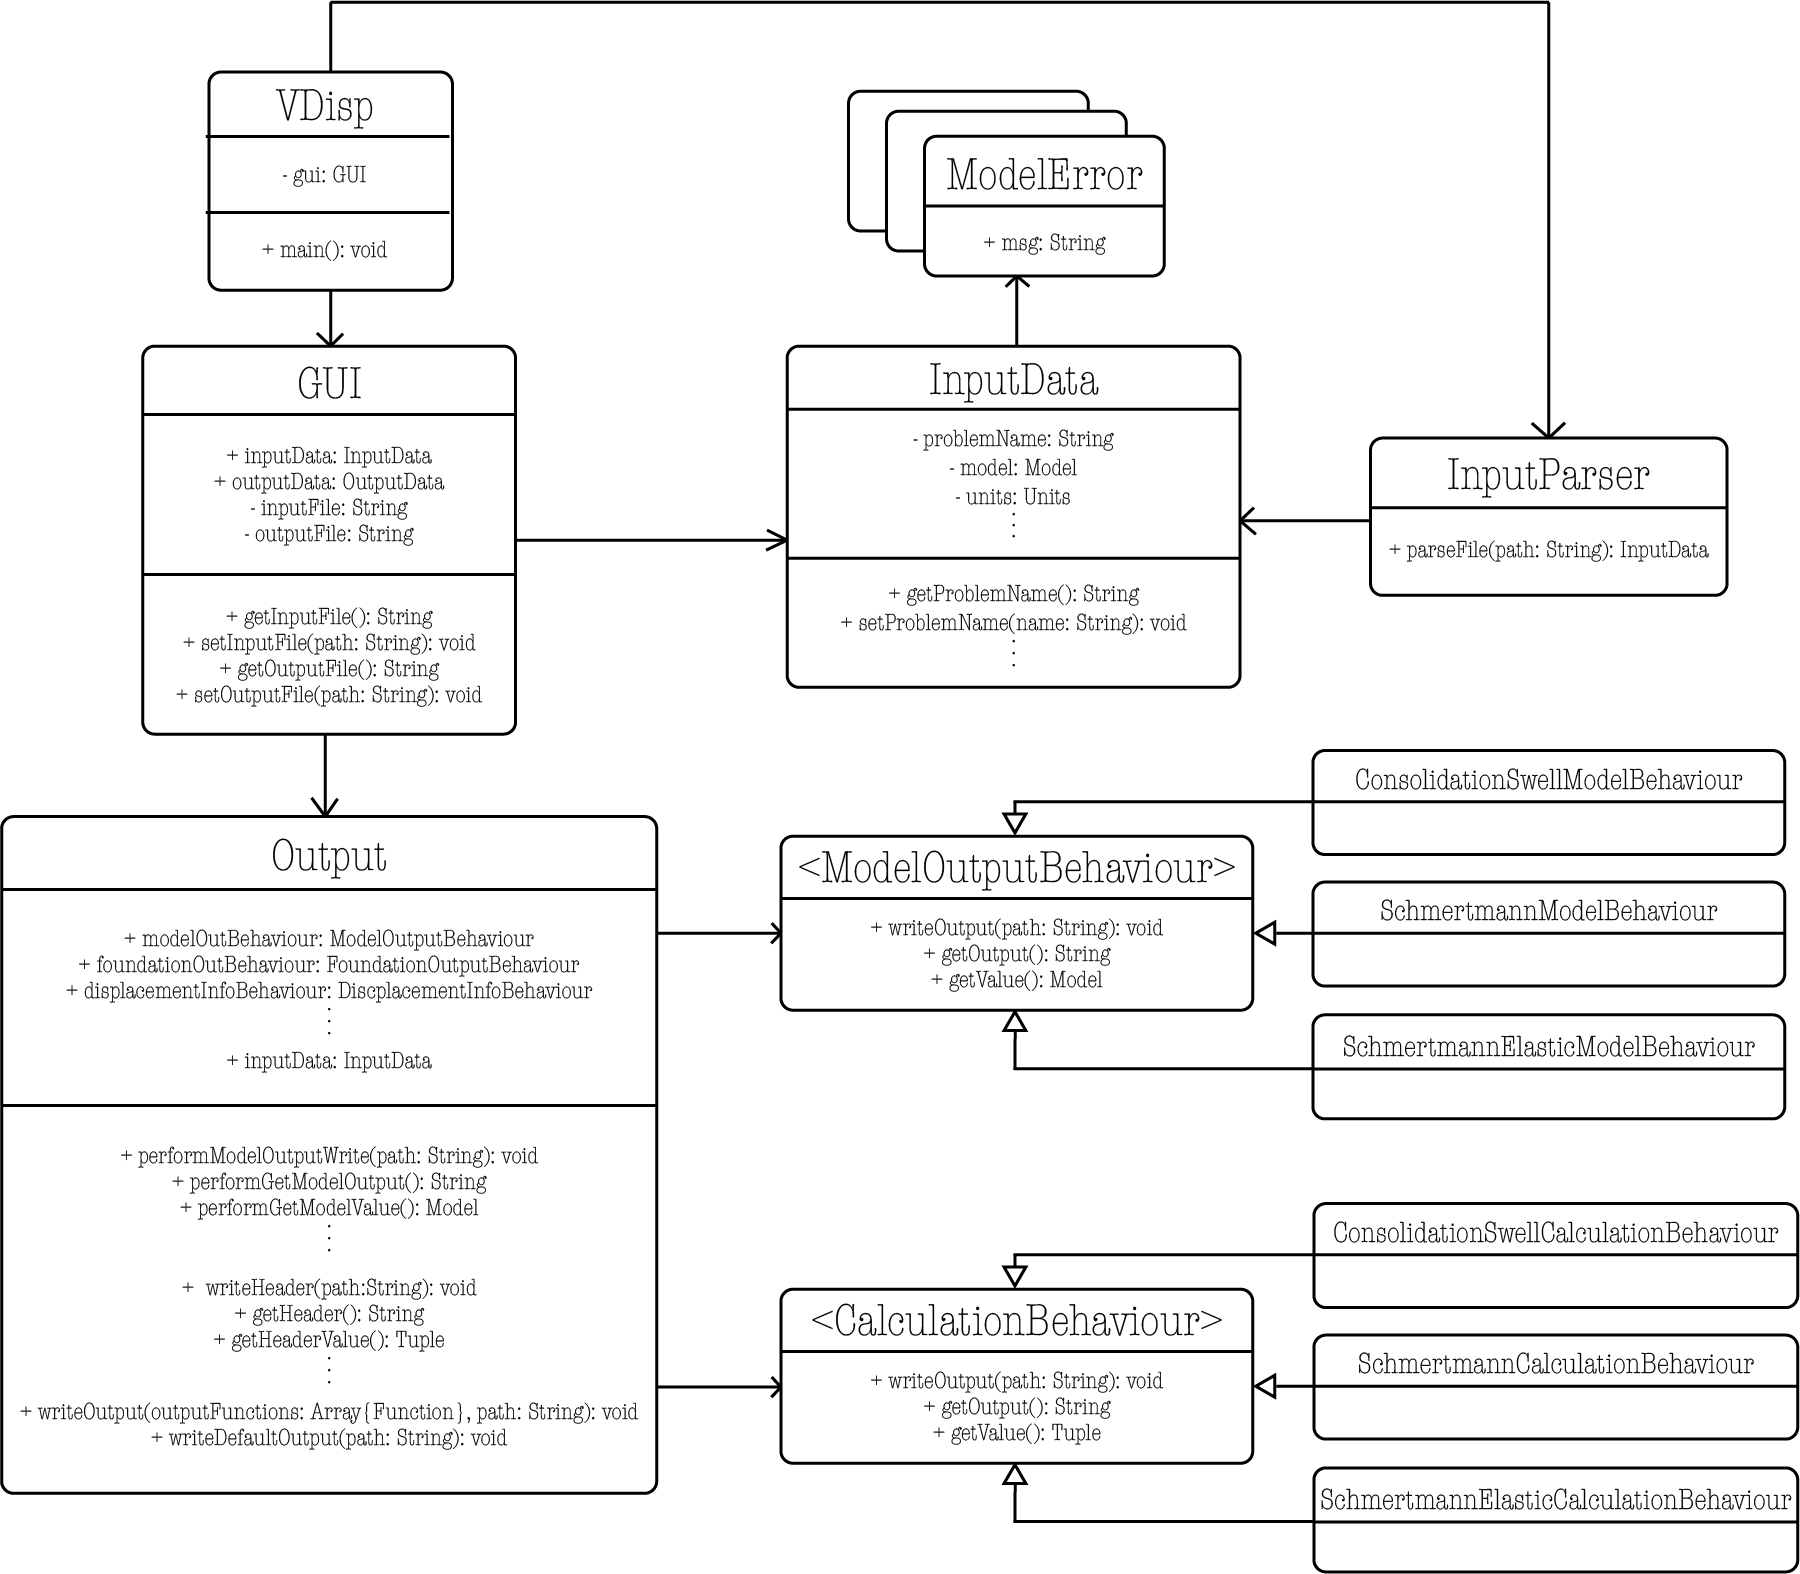
\includegraphics[width=1.3\textwidth]{VDispIdealDesignUML.png}
        \centering
    \end{figure}

    \indentpar The diagram above has been condensed. \emph{InputData} uses many 
    Custom Exception classes which help identify specific problems in the input file
    format allowing for helpful and descriptive messages to be given to the user. Furthermore,
    the \textbf{FoundationOutputBehaviour}, \textbf{DisplacementInfoBehaviour}, \textbf{ForcePointBehaviour} and
    \textbf{EquilibriumInfoBehaviour} interfaces (and the classes that implement them) have 
    been left out of the diagram. 
    
    \indentpar Examining the \textbf{ModelOutputBehaviour} interface is sufficient
    to understand the implementation of the excluded interfaces, while the \textbf{CalculationOutputBehaviour}
    is more complex than the other interfaces. The classes that implement \textbf{CalculationOutputBehaviour}
    are responsible for making method specific calculations, and return a set of values that is dependant on 
    the method itself. This is why the \textbf{CalculationOutputBehaviour} \emph{getValue()} function is said to
    return a \textbf{Tuple}. This \textbf{Tuple} contains different info based on the specified model, and classes
    that access this \textbf{Tuple} must be prepared to parse it.

    \indentpar The design pattern of the \emph{Output} class and the interfaces it uses (all the interfaces that 
    end in "\emph{Behaviour}") is inspired by the \emph{Duck example} in the opening chapter of \href{https://github.com/ksatria/MK-Design-Pattern/blob/master/Ebook/Head%20First%20Design%20Patterns.pdf}{this textbook}
    on design patterns.
    %%%%%%%%%%%%%%%%%%%%%%%%%%%%%%%%%%%%%%%%%%%%%%%%%%%%%%%%%%%%%%%
    
    %% Ideal Design %%%%%%%%%%%%%%%%%%%%%%%%%%%%%%%%%%%%%%%%%%%%%%%
    \section*{Actual Design} \label{actualDesign}

    \indentpar This section aims to describe the actual design which was implemented
    in the \textbf{VDisp} software. It strays from the \hyperref[initialDesign]{ideal design} due
    to some limitations outlined in the \hyperref[juliaLimits]{Julia Limitations} section.\\
    %%%%%%%%%%%%%%%%%%%%%%%%%%%%%%%%%%%%%%%%%%%%%%%%%%%%%%%%%%%%%%%
    
    %% Julia Limitations %%%%%%%%%%%%%%%%%%%%%%%%%%%%%%%%%%%%%%%%%%
    \section*{Julia Limitations} \label{juliaLimits}
    %%%%%%%%%%%%%%%%%%%%%%%%%%%%%%%%%%%%%%%%%%%%%%%%%%%%%%%%%%%%%%%

\end{document}